\section{Résultats}
\label{sec:resultats}

\subsection{Résultats de la première expérience}

Les résultats de la première expérience sont montrés dans la \figref{renaming}. Tout d'abord, le nombre de renommage varie beaucoup entre les projets. Par exemple, Jenkins a au plus $10\%$ de ses fichiers renommés dans la pire période alors que PHPUnit a deux périodes à plus de $50\%$. Le nombre de renommages varie aussi en fonction des périodes, par exemple dans PHPUnit la période $3.6 - 3.7$ a moins de $5\%$ de fichiers renommés alors que la période $3.7 - 4.0$ a presque $99\%$. En général, il y a beaucoup de périodes avec $0\%$ de fichiers renommés.\\

\begin{figure*}[h]
	\centering
	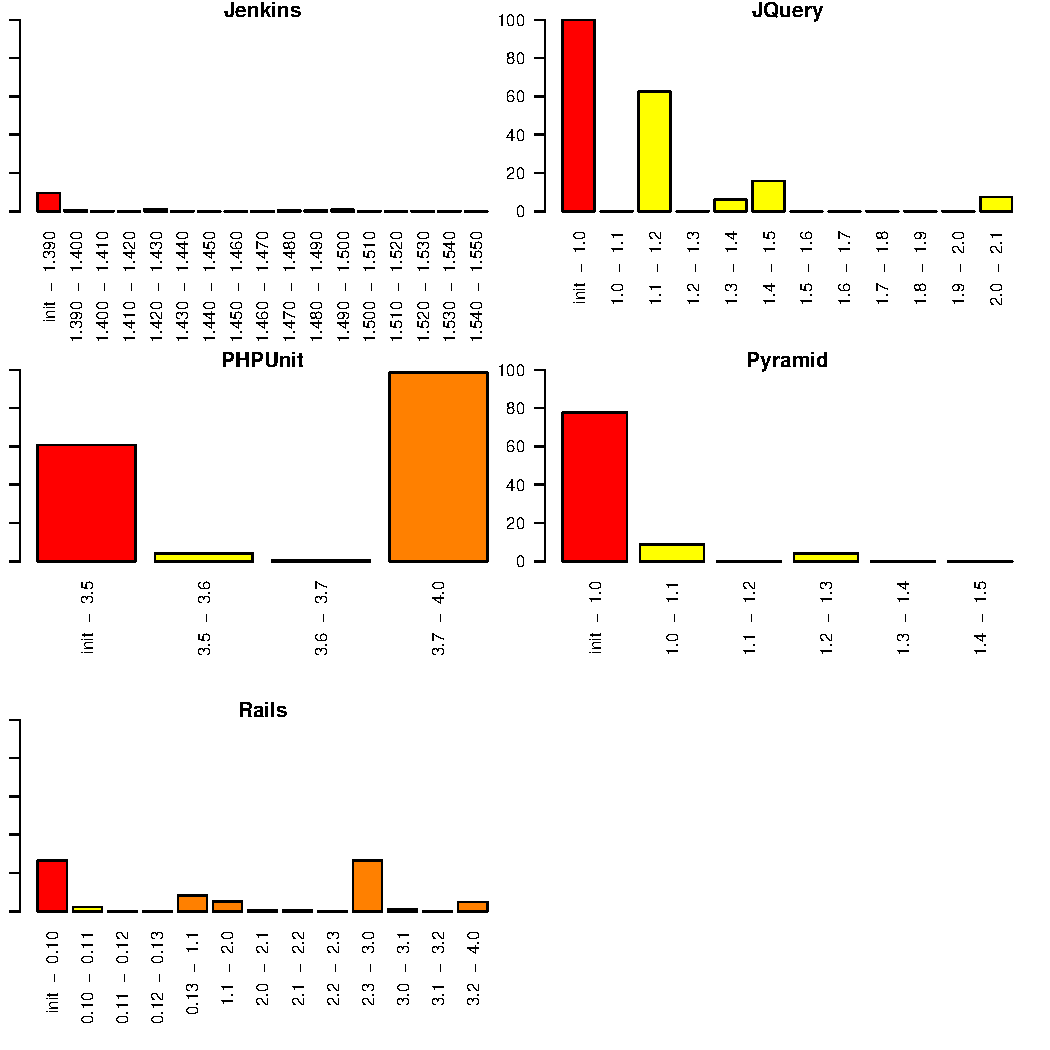
\includegraphics[width=0.85\linewidth,keepaspectratio]{data/figures/renaming.pdf}
	\caption{Pourcentage de fichiers renommés ($\%F_R$) dans chaque période de chaque projet de notre corpus. La période initiale est en gris foncé, les périodes majeures en gris et les périodes mineures en gris clair.}
	\label{fig:renaming}
\end{figure*}

Par rapport à la localisation de ces renommages, la période initiale semble la plus prolifique au renommage. En général, elle contient le plus grand nombre de fichiers renommés (sauf pour PHPUnit). Les périodes de développement sont plus susceptibles d'avoir des renommages que les périodes de maintenance. Ainsi, les $5$ projets sont quasiment à $0\%$ de fichiers renommés dans les périodes de maintenance (voir tableaux détails). Finalement, certaines périodes de développement peuvent contenir beaucoup de renommages. Les résultats montrent que les releases majeures sont souvent les pires périodes de développement en nombre de fichiers renommés: C'est le cas pour PHPUnit et Rails alors que Jenkins et Pyramid ne contiennent pas de releases majeures.\\

Le détail des résultats obtenus par notre outil de détection de renommage sont montrés dans les tables en annexes \tabref{jenkins}, \tabref{jquery}, \tabref{phpunit}, \tabref{pyramid} et \tabref{rails}. Ces tables mettent en avant les valeurs suivantes:\\

\begin{itemize}
\item \emph{Nombre de fichiers ($\#F$):} nombre de fichiers dans le projet à la dernière version de la période..
\item \emph{Nombre de fichiers actifs ($\#AF$):} nombre de fichiers créés, suprimés, copiés ou renommés durant la période et présents à la dernière version de la période.
\item \emph{Pourcentage de fichiers actifs ($\%AF$):} $\%AF = \frac{\#AF}{\#F}$.
\item \emph{Nombre de fichiers actifs renommés ($\#AF_{r}$):} nombre de fichiers actifs qui ont étés renommés.
\item \emph{Pourcentage de fichiers renommés ($\%F_{R}$):} $\%F_{R} = \frac{\#AF_{R}}{\#F}$.
\item \emph{Pourcentage de fichiers actifs renommés ($\%AF_{R}$):} $\%AF_{R} = \frac{\#AF_{R}}{\#AF}$.
\end{itemize}

\subsection{Résultats de la deuxième expérience}
Les résultats de notre deuxième expérience sont montrés dans la \tabref{spearman}. Ils montrent que la corrélation de coefficients de Spearman entre les métriques de procédés avec et sans détection de renommages dépendend beaucoup de la période et de la métrique choisie. Les métriques de procédés ne sont pas affectées par le renommage dans les projets Jenkins, Rails et Pyramid tels que le coefficient de corrélation est proche de $1$ dans tous les cas. D'un autre côté, pour PHPUnit et JQuery les métriques peuvent être sévèrement impactées par le renommage. Pour JQuery, la métrique Code Churn n'est pas affectée par le renommage, mais NoD et NoC sont quant à eux significativement impactés. Pour PHPUnit, toutes les métriques sont affectées par le renommage. Sur ces deux derniers projets, la métrique la plus sensible aux renommages de fichiers est le nombre de développeurs (NoD). Sur ces deux derniers projets, la métrique la plus sensible aux renommages de fichiers est le nombre de développeurs (NoD).

Finalement on peut noter que seules les périodes ayant eu un grand pourcentage de fichiers renommés ($\%F_R$) ont étés impactés. On peut aussi noter que des métriques biaisées par le renommage ont été calculées dans des releases majeures et mineures.\\

Nous avons étudié manuellement les deux périodes qui ont affecté les valeurs des métriques de procédés (JQuery 1.1 - 1.2 et PHPUnit 3.7 - 4.0). Par conséquent un grand nombre de fichiers ont étés renommés de manière transitive. C'est une pratique courante dans le développement logiciel, donc le phénomène pourrait apparaitre dans n'importe quelle période ou projet. Il est intéressent de noter que dans ces deux périodes les changements de structure ont été effectués en grande partie dans un seul commit proche de la fin de la période.\\


\begin{table*}[h]
\centering
\csvreader[tabular=rcccc, table head=\toprule & & \multicolumn{3}{c}{Change metrics}\\\cmidrule{3-5} Period & $\%F_R$ & CC & NoD & NoC\\\midrule, late after line=\\, late after last line=\\\bottomrule]{data/tables/correlations.csv}%
{1=\period,2=\fr,3=\churnall,4=\devall,5=\modificationsall}%
{\period & \fr & \churnall & \devall & \modificationsall}
\caption{La corrélation de coefficients de Spearman entre les valeurs des métriques de procédés avec et sans détection de renommage. Les codes de signification sont: *** $\leq 0.01$, ** $\leq 0.05$, * $\leq 0.1$ et ! $> 0.1$. Les coéfficiants moyen et faible sont affichés en gras.(TODO : gérer les tableaux)}
\label{tab:spearman}
\end{table*}


\subsection{vérifications}
